\cleardoublepage

\chapter{BASIC ASPECTS OF EXPOSURE TO ELECTROMAGNETIC FIELDS}
\label{chap:2}

\section{A Primer on Electromagnetic Fields}
An \gls{emf}, in a classical sense, i.e. non-quantum, is a concept denoting smooth motions of charged particles through space.
In classical electrodynamics, oscillating charges produce variations in the electric, $\mathcal{E}$, and magnetic, $\mathcal{H}$, field in a continuous manner where, in that case, energy is viewed as being transferred continuously through a field between any two distinct points in space~\cite{Griffiths2017Introduction}.
A simple visual representation of a plane wave, whose value, at any moment, is constant through any plane that is perpendicular to a fixed direction in space~\cite{Brekhovskikh1980Waves}, is shown in \cref{fig:EMWave}.
% source: https://tex.stackexchange.com/a/229678
\begin{figure}[b]
    \centering
    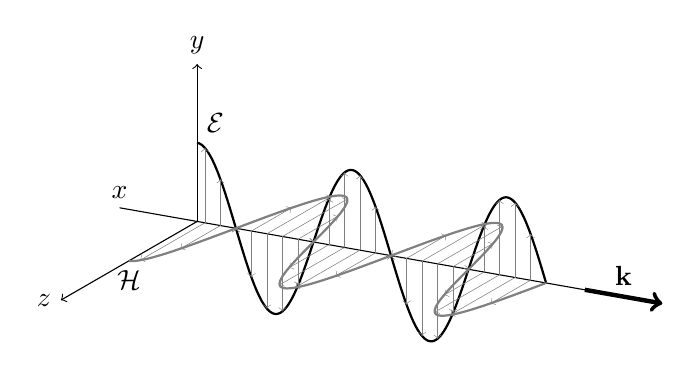
\begin{tikzpicture}[x={(-10:1cm)},y={(90:1cm)},z={(210:1cm)}]
        % Axes
        \draw (-1,0,0) node[above] {$x$} -- (5,0,0);
        \draw[->] (0,0,0) -- (0,2,0) node[above] {$y$};
        \draw[->] (0,0,0) -- (0,0,2) node[left] {$z$};
        % Propagation
        \draw[->,ultra thick] (5,0,0) -- node[above] {$\mathbf{k}$} (6,0,0);
        % Waves
        \draw[thick] plot[domain=0:4.5,samples=200] (\x,{cos(deg(pi*\x))},0);
        \draw[gray,thick] plot[domain=0:4.5,samples=200] (\x,0,{cos(deg(pi*\x))});
        % Arrows
        \foreach \x in {0.1,0.3,...,4.4} {
          \draw[->,help lines] (\x,0,0) -- (\x,{cos(deg(pi*\x))},0);
          \draw[->,help lines] (\x,0,0) -- (\x,0,{cos(deg(pi*\x))});
        }
        % Labels
        \node[above right] at (0,1,0) {$\mathcal{E}$};
        \node[below] at (0,0,1) {$\mathcal{H}$};
    \end{tikzpicture}

    \caption{A plane wave propagating in free space with a direction defined by the wave vector perpendicular to the wave front.}
    \label{fig:EMWave}
\end{figure}

The number of oscillations per unit time is referred to as the frequency, $f$, of the field.
The quantum picture of \gls{emf}s is somewhat different: the moving charged particles are treated as ``quantum harmonic oscillators'' described via \gls{emf} tensors.

Mathematically, \gls{emf}s are formulated within the Maxwell framework originally consisted of twenty scalar equations and subsequently reduced to four partial differential vector equations~\cite{Hampshire2018derivation}.
These equations encapsulate the relationship between fields and their sources in a symmetric form~\cite{Poljak2006Advanced}
\begin{align}
    \label{eqn:maxwell-faraday}
    \nabla \times \mathcal{E} &= -\frac{\partial \mathcal{B}}{\partial t},\\
    \label{eqn:maxwell-ampere}
    \nabla \times\mathcal{H} &= \mathcal{J} + \frac{\partial \mathcal{D}}{\partial t},\\
    \label{eqn:maxwell-gauss}
    \nabla \cdot \mathcal{D} & = \rho,\\
    \label{eqn:maxwell-gauss-magnetics}
    \nabla \cdot \mathcal{B} &= 0.
\end{align}

The differential form of the Faraday law is expressed in~\cref{eqn:maxwell-faraday}, which indicates that the time-varying magnetic flux density, $\mathcal{B}$, is the source of the rotating electric vector field, $\mathcal{E}$.
\Cref{eqn:maxwell-ampere} presents an expanded differential formulation of the Ampere law.
It asserts that electric current density, $\mathcal{J}$, acts as the source of the rotating magnetic vector field, $\mathcal{H}$.
To ensure consistency with the law of conservation of electric charge, the concept of displacement currents is introduced through the time-varying electric flux density, $\mathcal{D}$.
In \cref{eqn:maxwell-gauss}, the Gauss law establishes the relationship between static electric fields and electric charges. A static electric field points from positive charges towards negative charges, with the net field outflow being proportional to the charge in a bounded volume of space.
Conversely, the Gauss law for magnetism, which stipulates the absence of magnetic monopoles, is given in~\cref{eqn:maxwell-gauss-magnetics}.

As the field propagates away from a source, it transfers energy from its source to the surrounding space.
The general conservation of energy for a configuration consisting of electric and magnetic fields acting on charges is given by the Poynting theorem.
This theorem establishes an energy equilibrium by stating that the rate at which energy is transferred (per unit volume) from a specific region of space equals the combined effect of the work performed on the charges within that volume and the energy flux leaving the region~\cite{Jackson1998Classical}.
The integral form of the Poynting vector is given by
\begin{align}
    \label{eqn:poynting-theorem}
    \int_{V} \mathcal{E}' \cdot \mathcal{J} \mathrm{d}V = \frac{\partial}{\partial t}\int_V \frac{1}{2} \; \left( \mathcal{E} \cdot \mathcal{D} + \mathcal{H} \cdot \mathcal{B} \right) \; \mathrm{d}V + \int_{V} \frac{\left| \mathcal{J} \right|}{\sigma} \; \mathcal{J} \; \mathrm{d}V \oint_S \left( \mathcal{E} \times \mathcal{H} \right) \; \mathrm{d} \mathbf{S} = 0,
\end{align}
where $\sigma$ represents the density of the material bounded by the surface.
Herein, the sources within the volume of interest, characterized by electric field $\mathcal{E}'$, are balanced with the rate of increase of \gls{em} energy in the domain, the rate of flow of energy in through the domain surface and the Joule heat production within the domain, respectively.
The flow of energy through the surface, $S$, bounding the observed volume in a unit of time is defined as
\begin{align}
    \label{eqn:poynting-theorem-energy}
    \oint_S \left( \mathcal{E} \times \mathcal{H} \right) \; \mathrm{d} \mathbf{S}.
\end{align}
Within \cref{eqn:poynting-theorem-energy}, the time-varying vector field, i.e., the Ponyting vector,
\begin{align}
    \label{eqn:poynting-vector}
    \mathcal{P} = \mathcal{E} \times \mathcal{H},
\end{align}
represents the power density vector which defines the direction of the \gls{emf} at any point in space.

For the time-harmonic quantities, the complex Poynting vector is given by
\begin{align}
    \mathbf{P} = \frac{1}{2} \; \left( \mathbf{E} \times \mathbf{H}^* \right)
\end{align}
Then, the steady state flow of energy through the surface, $S$, is defined as
\begin{align}
    \oint_S \left( \mathbf{E} \times \mathbf{H}^* \right) \; \mathrm{d} \mathbf{S} = &-j \; \frac{\omega}{2} \; \int_V \left( \mu \; \left| \mathbf{H} \right|^2 - \varepsilon \; \left| \mathbf{E}^2 \right|^2 \right) \; \mathrm{d}V \\ \notag
    &- \frac{1}{2} \; \int_V \sigma \; \left| \mathbf{E} \right|^2 \; \mathrm{d}V + \frac{1}{2} \; \int_V \sigma \; \left| \mathbf{E}' \right|^2 \; \mathrm{d}V,
\end{align}
where $j$ represents the unit imaginary number, $\varepsilon$ stands for the absolute permittivity and $\mu$ is the magnetic permeability.
The real part of the above expression represents the total averaged power while the imaginary part of the integral of the Poynting vector is proportional to the difference between averaged stored magnetic energy in the volume and averaged stored energy in the electric field.
The factor of $\nicefrac{1}{2}$ appears as \gls{emf} components are given as peak values and it is omitted for the \gls{rms} values.

\section{Principles of Non-Ionizing Radiation Effects on Tissue}
\gls{em} radiation arises from periodic alterations in electric and/or magnetic fields, resulting in the generation of distinct wavelengths across the \gls{em} spectrum.
The frequency and wavelength of these waves are reciprocally related, with the propagation speed of waves in space acting as the constant of proportionality.
In a vacuum, where interactions with scatterers are absent, \gls{em} waves travel at the speed of light.
Conversely, in lossy medium, the speed is reduced.
\Gls{emf}s can impact upon material which results in the interaction with atoms and molecules in that material.
Resulting effects depend on the power, frequency, and wavelength of the field, as well as the physical properties and dimensions of the interacting material.

Non-ionizing \gls{em} radiation, characterized by photon energy up to \SI{10}{\eV}, lacks sufficient energy contained in a single photon to ionize atoms or molecules by removing their most weakly bound electrons.
It is categorized into wavelength/frequency bands: \gls{uv} (\SIrange{100}{400}{\nm}), visible light (\SIrange{400}{780}{\nm}), \gls{ir} (\SIrange{780}{1000}{\nm}), \gls{rf} \gls{emf}s (\SI{100}{\kHz} up to \SI{300}{\GHz}), \gls{lf} (\SI{1}{\Hz} up to \SI{100}{\kHz}) and static electric and magnetic fields.
However, despite photons being electrically neutral, they are able to indirectly induce ionization in the matter via mechanism, such as the photoelectric effect and Compton effect, that are out of the scope of the thesis.
It is generally accepted that indirectly ionizing radiation occurs when energy of a single photon is greater than \SI{10}{\eV} which corresponds to the higher energy region of the \gls{uv} spectrum (wavelength of \SI{124}{\nm} or lower)~\cite{ARPANSA2023What,Bulletin1999QuestionsAA}.
Thus, ionizing radiation encompasses high-energy \gls{uv} radiation, X-rays, and gamma rays.
Refer to~\cref{fig:EMSpectrum} for a visual representation of the \gls{em} spectrum.
% source: https://tex.stackexchange.com/a/498765
\pgfdeclarehorizontalshading{visiblelight}{50bp}{% https://tex.stackexchange.com/a/348492/120853
    color(0bp)=(violet!25);
    color(8.33bp)=(blue!25);
    color(16.67bp)=(cyan!25);
    color(25bp)=(green!25);
    color(33.33bp)=(yellow!25);
    color(41.5bp)=(orange!25);
    color(50bp)=(red!25)
}%

\begin{figure}[t]
    \centering
    \begin{tikzpicture}[%
            raylabel/.style={font=\scriptsize}
        ]
        \def\minexponent{-6}
        \def\maxexponent{6}
        \def\spectrumheight{9em}
    
        \pgfmathtruncatemacro{\nextminexponent}{\minexponent + 1}
    
        % Main foreach loop, drawing the wavelengths as powers of 10 in an alternating fashion: even on top, odd at bottom. Then connects them with help lines
        \foreach [count=\i, remember=\exponent as \previousexponent, evaluate=\i as \currentposition using int(\i/2)] \exponent in {\minexponent, \nextminexponent, ..., \maxexponent}{
            \ifodd\exponent
                \def\height{0}
            \else
                \def\height{\spectrumheight}
            \fi
    
            % Anchor at baseline to get all nodes on same baseline.
            % https://tex.stackexchange.com/questions/133227/how-to-align-text-in-tikz-nodes-by-baseline#comment300863_133227
            \node[anchor=base] (WAVELENGTH_\exponent) at (\exponent, \height) {\contour{white}{\num{e\exponent}}};
    
            \ifnum\i > 1
                \ifodd\i
                    \node (LABEL_\currentposition)
                        at ($(WAVELENGTH_\exponent)!0.5!(WAVELENGTH_\previousexponent)$)
                        {};% This is left as a node as opposed to coordinate: fill it out with '\currentposition' for debugging
                \else
                    % Do not draw connection at exponent 1:
                    \pgfmathparse{\exponent != 1}% \pgfmathparse stores result (0 or 1) in macro \pgfmathresult
                    \ifnum\pgfmathresult = 1
                        \draw[help lines]
                            (WAVELENGTH_\previousexponent) --(WAVELENGTH_\exponent)
                            node[midway] (CONNECTION_\currentposition) {}% This is left as a node as opposed to coordinate: fill it out with '\currentposition' for debugging
                            coordinate[at start] (CONNECTION_\currentposition_START)
                            coordinate[at end] (CONNECTION_\currentposition_END);
                    \fi
                \fi
            \fi
        }
    
        % Create an arrow shape that fits around all relevant nodes, but do not draw it.
        % Draw it manually later to leave out the 'bottom' of the arrow.
        % We still need this invisible arrow for lining up of coordinates
        \node[
            single arrow,
            single arrow head extend=0pt,
            single arrow tip angle=150,% Inner angle of arrow tip
            fit={([xshift=-3em]CONNECTION_1_START)(CONNECTION_1_END)(CONNECTION_\maxexponent_START)([xshift=5em]CONNECTION_\maxexponent_END)},
            inner sep=0pt
        ]
        (ARROW) {};
    
        % On background layer so already drawn arrow and scale lines cover it up nicely
        \begin{scope}[on background layer]
            \node[
                inner sep=0pt,
                outer sep=0pt,
                fit={([xshift=-2.2em]WAVELENGTH_0|-ARROW.after tail)([xshift=-2.2em]WAVELENGTH_1|-ARROW.before tail)}, shading=visiblelight]
                (SMALL_VISIBLE_LIGHT) {};
    
            \shade[
                left color=white,
                right color=violet!25,
                middle color=violet!5,
                outer sep=0pt
                ]
                (CONNECTION_3_START) -- (CONNECTION_3_END) -- ([xshift=\pgflinewidth]SMALL_VISIBLE_LIGHT.south west) -- ([xshift=\pgflinewidth]SMALL_VISIBLE_LIGHT.north west) -- cycle;
    
            \shade[
                left color=red!25,
                right color=white,
                middle color=red!5,
                outer sep=0pt,
                ]
                (CONNECTION_5_START) -- (CONNECTION_5_END) -- ([xshift=-\pgflinewidth]SMALL_VISIBLE_LIGHT.south east) -- ([xshift=-\pgflinewidth]SMALL_VISIBLE_LIGHT.north east) -- cycle;
        \end{scope}
    
        % Some labels can be drawn automatically at the designated label coordinates:
        \foreach [count=\i] \label in {
                {gamma\\rays},
                {X-rays},
                {},%Skip this one
                {IR}
            }{
                \node[raylabel, align=center] at (LABEL_\i) {\label};
            }
    
        % These do not fit the loop and are drawn manually:
        \node[raylabel, anchor=north] at ([yshift=-3.85em]$(WAVELENGTH_-2)!0.45!(WAVELENGTH_0)$) {UV};
    
        \node[raylabel, fill=white, align=center] at (CONNECTION_6) {\gls{rf}\\radiation};
    
        \node[raylabel, right=3em of CONNECTION_6, align=right] {LF\\radiation};
    
        \node[raylabel, left=1em of CONNECTION_1, align=left] {cosmic\\rays};
    
        \node[
            draw,
            fill=black!20,
            below=4em of SMALL_VISIBLE_LIGHT,
            align=center,
            label=above:{\textbf{visible light}}
            ] (FULL_VISIBLE_LIGHT) {%
            \pgfspectra[width=13em,height=3em]\\%pgfspectra also has a builtin axis which of course much better than this terrible approach, but it is in nanometer
                {\SI{0.40}{} \hfill \SI{0.48}{} \hfill \SI{0.58}{} \hfill \SI{0.68}{} \hfill \SI{0.78}{\um}}
        };
    
        % Draw 'magnifying' trapeze, on background so it is covered by scale labels
        \begin{scope}[on background layer]
            \filldraw[help lines, fill=black!10] (FULL_VISIBLE_LIGHT.north east) -- (SMALL_VISIBLE_LIGHT.south east) -- (SMALL_VISIBLE_LIGHT.south west) -- (FULL_VISIBLE_LIGHT.north west) -- cycle;
        \end{scope}
    
        % Draw around arrow manually, leaving its tail open
        \draw[draw, thick] (ARROW.after tail) -- (ARROW.before head) -- (ARROW.before tip) -- (ARROW.tip) -- (ARROW.after tip) -- (ARROW.after head) -- (ARROW.before tail);
    \end{tikzpicture}
    
    \caption{Diagram of the electromagnetic spectrum as a function of wavelengths.}
    \label{fig:EMSpectrum}
\end{figure}

Non-ionizing \gls{em} waves interact with material in space, transferring kinetic energy to bounded atoms and molecules, thereby increasing their vibration rate and raising the temperature in the affected region.
However, this effect is only observed when the wavelength of incident waves is of the same order of magnitude as the dominant dimension of the irradiated material.
Conditioned by the interaction of non-ionizing radiation and biological tissue, a biological effect can be described as any biological, physical, or chemical change induced in this tissue~\cite{ICNIRP2020Principles}.
Living organisms have repair and feedback mechanisms intended primarily for preservation of homeostasis.
Once upper threshold limits in the capacity of these mechanisms are exceeded, adverse health effects may occur.
In some cases, the difference between the biological and adverse health effect is not clear as it may vary significantly upon individual's perception and sensitivity.
Distinguishing adverse health effects from other biological effects aligns with the World Health Organization's definition of health, which emphasizes complete physical, mental, and social well-being rather than mere absence of disease or infirmity~\cite{WHO2022Health}.
If a biological perception arises as a result of non-ionizing radiation (e.g., tingling sensation~\cite{Saunders2007neurobiological}, magnetophosphenes~\cite{Lövsund1980Magnetophosphenes}, microwave hearing~\cite{Frey1962Human}) without negatively impacting an individual's health, it is not considered as an adverse health effect~\cite{ICNIRP2020Principles}.

The interaction between non-ionizing radiation and biological tissue can result in thermal and non-thermal effects.
Non-thermal effects, such as nerve stimulation, are typically associated with \gls{lf} radiation up to \SI{100}{\kHz}, while thermal effects are predominantly observed above \SI{10}{\MHz}.
\Cref{tab:interaction-mechanism} provides an overview of the bioeffects in the non-ionizing \gls{em} spectrum.
\begin{table}[b]
    \centering
    \caption{Summary of the effects of non-ionizing radiation on biological tissues.}
    \label{tab:interaction-mechanism}
    \resizebox{\textwidth}{!}{%
        \begin{tabular}{|c|c|c|}
            \hline \textbf{exposure to}  & \textbf{frequency range} & \textbf{bioeffect} \\
            \hline static magnetic fields & \SI{0}{\Hz} & induced electric fields and current \\
            \hline \gls{lf} radiation & \SI{1}{\Hz} to \SI{100}{\kHz} & stimulation of excitable cells \\
            \hline & \SI{100}{\kHz} to  \SI{10}{\MHz} & stimulation of excitable cells and tissue heating \\
            \cline{2-3} \multirow{-2}{*}{\gls{rf} radiation} & \SI{100}{\MHz} to \SI{300}{\GHz} & \\
            \cline{1-2} \gls{ir} radiation & \SI{300}{\GHz} to  $\sim$ \SI{400}{\THz} & \\
            \cline{1-2} visible light & $\sim$ \SI{400}{\THz} to  $\sim$ \SI{790}{\THz} & \\
            \cline{1-2} low energy \gls{uv} & above \SI{790}{\tera\Hz} & \multirow{-4}{*}{tissue heating} \\
            \hline
        \end{tabular}%
    }
\end{table}
Exposure to \gls{emf}s induces electric fields within tissue, which can stimulate any excitable cells of that tissue up to \SI{10}{\MHz}~\cite{Saunders2007neurobiological}.
Pulsed \gls{emf}s of sufficient intensity at low frequency can alter cell membrane permeability and cause deformation of intracellular structures when the duration of exposure is shorter than the charging time of the outer membrane~\cite{Joshi2010Critical}.
As the frequency increases, heating effects predominate and the likelihood of nerve stimulation drastically decreases.
However, evidence suggests the existence of non-thermal effects above \SI{100}{\MHz}, which are manifested as changes in cell membrane activity, transmembrane potentials, and the cell cycle~\cite{Romanenko2017interaction}.
Since there is no consensus on their adversity with regards to the tissue health, they fall out of the scope of this thesis.
It is nevertheless important to note that in~\cite{Fröhlich1968Long}, theoretical predictions of the existence of megahertz to terahertz oscillations in living cells have raised interest in the risks and potentials of \gls{emf}s and tissues.
Extensive reviews have explored physiological, cellular, and molecular-level biological effects at \gls{mmw}~\cite{Pakhomov1998Current,Zhadobov2011Millimeter}.
Some arguments support possible interactions with living organisms, excluding direct and indirect thermal effects, such as therapeutic applications~\cite{Ziskin2006Physiological}.
However, it remains unclear if these effects can be fully understood without considering them within the context of the thermodynamics framework.

\section{Radio-Frequency Electromagnetic Radiation Protection}
The development and widespread use of electronic systems have led to increased human exposure to artificial \gls{emf}s~\cite{Hirata2021Assessment}.
Consumer electronics, primarily in the \gls{rf} portion of the \gls{em} spectrum, are commonly used for communication, wireless information transmission, and wireless power transfer.
To ensure safe usage, regulatory international bodies, such as the \gls{icnirp} and \gls{ieee} \gls{ices}, have established guidelines~\cite{ICNIRP2020Guidelines} and standards~\cite{IEEE2019Standard}, respectively, to limit exposure for both the general public and individuals in restricted environments.

The exposure limits consider short- and long-term, continuous and discontinuous \gls{rf} \gls{emf} exposure, providing a high level of protection against adverse health effects~\cite{ICNIRP2020Guidelines,IEEE2019Standard}.
The limits are derived from scientific literature that classifies the effects of \gls{rf} \gls{emf} exposure on biological systems and tissues as potentially harmful.
They are identified as adverse health effect thresholds~\cite{ICNIRP2020Guidelines} or exposure limits~\cite{IEEE2019Standard}.
Reduction factors~\cite{ICNIRP2020Guidelines} or safety margins~\cite{IEEE2019Standard} are applied to these thresholds/limits, considering individual variability and variations in exposure setups and environments.

The resulting threshold values, incorporating reduction factors or safety margins, are expressed as in terms of \gls{br}s~\cite{ICNIRP2020Guidelines} or \gls{drl}s~\cite{IEEE2019Standard}.
They relate to physical dosimetric quantities, either peak or averaged in time and space, that are well correlated with occurrence of harmful impact as a result of \gls{rf} \gls{em} exposure.
To facilitate the assessment of exposure in situations where the aforementioned physical quantities are difficult to measure, \gls{rl}s~\cite{ICNIRP2020Guidelines} or \gls{erl}s~\cite{IEEE2019Standard} have been derived upon \gls{br}s or \gls{drl}s under worst-case exposure conditions.
This approach ensures a high degree of conservatism and facilitates compliance assessment with the exposure limits in a more practical manner.

\subsection{Brief History of Exposure Limits}
Since the establishment of the first commercial radio station, there has been a growing interest in assessing human exposure to \gls{rf} \gls{em} radiation.
The scientific investigation of the interaction between RF waves and human tissue began in the 1920s, driven by the increased use of \gls{rf} diathermy for therapeutic tissue heating~\cite{Kovacs1945Electrotherapy}.
In the 1950s, the U.S. Department of Defense initiated the Tri-Service Program to examine the potential impact of radiated fields on the human body as high-power \gls{rf} transmitters were operated in close proximity to personnel~\cite{Lin1994Early}.

During the 1970s, research in this area improved in quality~\cite{Guy1971Analyses}, but there was a public distrust due to the lack of concrete limits and regulations for the safety of wireless electronic devices in close proximity to the human body, leading to many controversies~\cite{Foster2022Three}.
Computational dosimetry studies, mostly focused on far-field exposure to plane-wave radiation, increased in response, culminating in the publication of dosimetry handbooks sponsored by the U.S. Air Force~\cite{Durney1986Radiofrequency}.
Simultaneously, comprehensive studies on environmental \gls{rf} fields in urban areas proliferated~\cite{Tell1976Measurement}, resulting in numerous surveys measuring \gls{rf} \gls{emf}s from various technologies in different exposure scenarios~\cite{Jalilian2019Public}.
The first formal \gls{rf} safety standards in the U.S were published in the late 1960s, from which the \gls{ieee} family of exposure standards (C95.1-x) emerged.
These early limits were primarily based on canonical models predicting whole-body heating and expressed in terms of \gls{ipd}~\cite{Roach2009Radiofrequency}.

Over the years, independent regulatory bodies such as the American National Standards Institute, \gls{icnirp}, and \gls{ieee} have developed their own standards.
While discrepancies between \gls{ieee} C.95.1-x standard and \gls{icnirp} guidelines existed~\cite{Repacholi2017history}, harmonization has mostly been achieved with the latest updates in 2019 and 2020~\cite{Foster2022Three}.
Advancements have been made by including high-fidelity \gls{em} simulation software, \gls{3-d} models for simulations, and accurate instruments for \gls{rf} exposure assessment.

During the last decade, research has doubled on all fronts: from experimental to epidemiological to dosimetric/technical studies.
However, the greatest progress can be seen in the quality and number of published studies carried out in computational dosimetry research, the main idea of which is the realization of precise simulations at high frequencies in the near-field~\cite{Diao2021Effect}.
This progress is driven by the emergence of new wireless communication devices based on \gls{5g}, utilizing higher parts of the \gls{rf} spectrum and advanced antenna technologies.
However, the availability of accurately measured experimental data, particularly at \gls{mmw}, remains limited, and existing studies do not provide sufficient information for safety assessment~\cite{Simkó20195G}.
The advancement of numerical methods and computing power~\cite{Poljak2018conformal}, and publicly available databases on the dielectric properties of human and animal tissues~\cite{Gabriel1996Compilation} have facilitated progress in computational bioelectromagnetics in general.
To put this in the frame of reference, \cref{fig:research_compilation} illustrates the evolution of research in \gls{rf} and mobile communications exposure assessment and dosimetry from 1950 to 2022.
\begin{figure}[t]
    \centering
    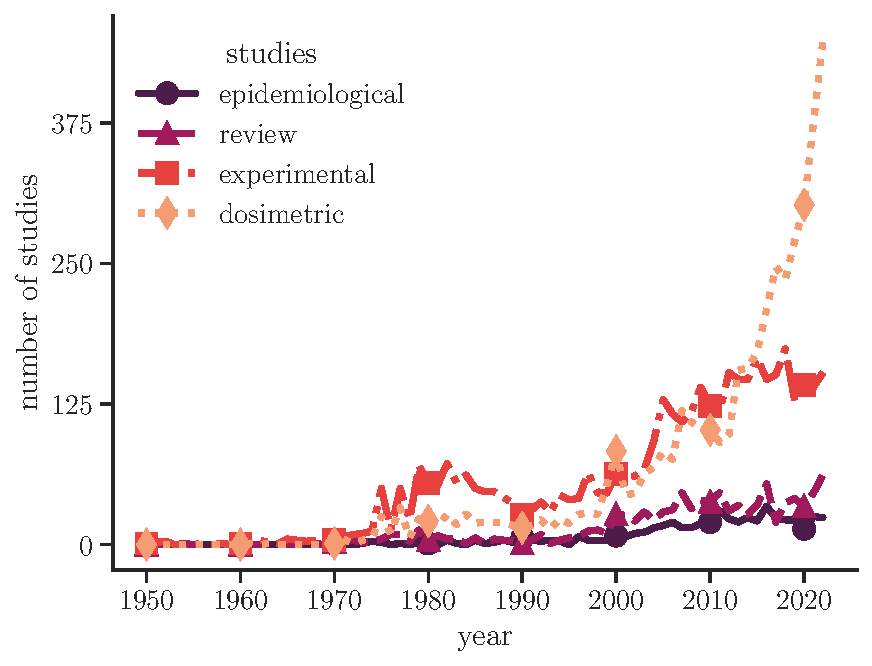
\includegraphics[width=0.8\textwidth]{artwork/research_compilation.pdf}
    \caption{Papers published between 1950 and 2022 related to research on bioeffects of radio-frequency electromagnetic fields and/or mobile communications.
    Compiled from \href{http://www.emf-portal.org}{\url{emf-portal.org}}.}
    \label{fig:research_compilation}
\end{figure}

\subsection{Scientific Basis for Limiting Exposure}
Below \SI{10}{\MHz}, induced electric fields may stimulate nerves and potentially cause dielectric breakdown of biological membranes~\cite{Swicord2008Has}.
Such and similar effects are defined as non-thermal and can be classified into four groups: resonance mechanisms, coupling with nonlinear systems, effects due to the direct action of electric and magnetic fields, and cooperative mechanisms due to interactions among several membrane components~\cite{DInzeo2009Deliverable}.
Above \SI{100}{\kHz}, the result of the interaction between induced electric fields and polar molecules or free charges within the exposed body is the kinetic energy which causes polar molecules to rotate and oscillate around their center and charges to form the electric current.
The increased kinetic energy leads to more frequent interactions and the conversion of kinetic energy into thermal energy~\cite{Foster2018Modeling}.

To evaluate heating effects, quantifying the absorbed power in exposed tissue is crucial.
It is generally considered that below \SI{6}{\GHz}, \gls{emf}s penetrate deep, whereas above this frequency, power is primarily dissipated on the surface of the tissue~\cite{Ziskin2018Tissue}.
\Cref{fig:penetration_depth} illustrates the power transmission coefficient and power penetration depth into a uniform half-plane of tissue with frequency-dependent dielectric properties of dry skin.
\begin{figure}[t]
    \centering
    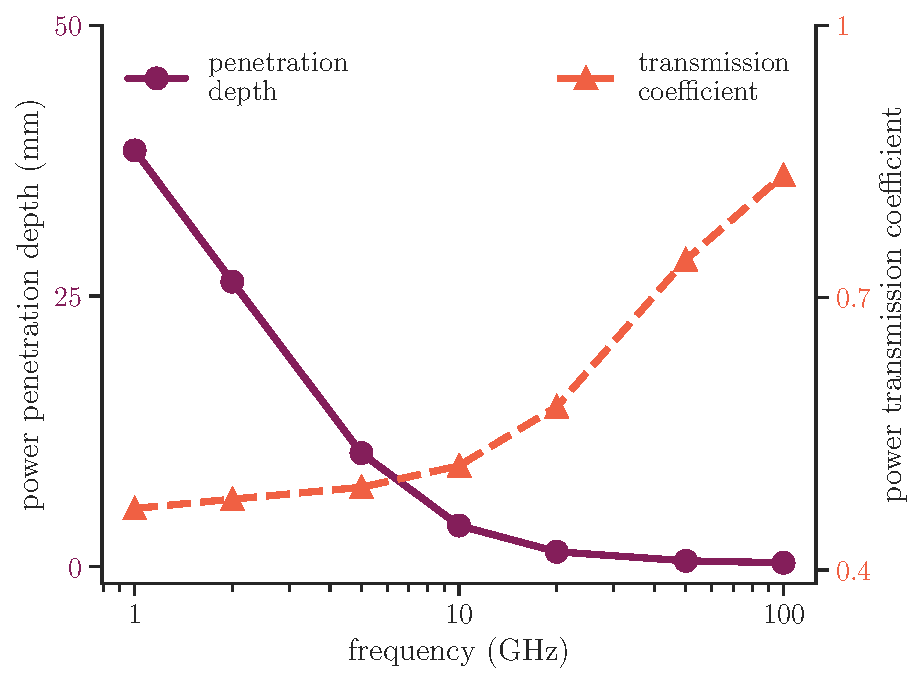
\includegraphics[width=0.8\textwidth]{artwork/penetration_depth.pdf}
    \caption{Power transmission coefficient and power penetration depth into dry skin as a function of frequency.}
    \label{fig:penetration_depth}
\end{figure}
Dielectric properties of dry skin are obtained from~\cite{Gabriel1996Compilation}.
The power penetration depth into the tissue is defined
as the distance beneath the surface at which the power density has fallen to a factor of $\nicefrac{1}{e}$ compared to the surface level, which is a half of the commonly reported wave penetration depth~\cite{Foster2016Thermal}.

Exposure limits set (operational) threshold levels to restrict temperature rise rather than focusing on absolute temperature.
Absolute temperature depends on various factors such as sex, age, thermoregulation, surrounding temperature, clothing, and work rate, which are not addressed by neither the \gls{icnirp} guidelines nor \gls{ieee} standard.
Temperature rise can be classified into steady-state and brief temperature rise.
Steady-state temperature rise gives sufficient time for heat to disperse throughout a larger tissue mass and for thermoregulatory processes to activate.
The steady-state increase of core body temperature is typically restricted to \SI{1}{\celsius}, although there is no scientific evidence for adversity even at higher temperature rise.
Due to the limited literature available, steady-state temperature rise of \SI{1}{\celsius} has been adopted in a conservative manner as it triggers significant physiological changes~\cite{Heuvel2017independent}, which are not represented as adverse health effects.

Furthermore, guidelines also specify limits for steady-state local temperature rise in specific body regions, such as the head, torso, and limbs.
For regions with normothermal temperature of \SIrange{33}{36}{\celsius}, the local temperature rise should be limited to \SI{5}{\celsius}.
In regions with higher normothermal temperature of \SIrange{36}{38.5}{\celsius}, such as the head, eyes, abdomen, thorax, and pelvis, the local temperature rise should be limited to \SI{2}{\celsius}.
These limits are based on experimental human studies~\cite{Walters2000Heating}, considering that tissue damage may occur at temperatures between \SIrange{41}{43}{\celsius}~\cite{Dewhirst2003Basic}, with the severity and likelihood of damage increasing with longer exposure times.

Lastly, rapid temperature rise can lead to inhomogeneous temperature distribution over the exposed tissue before thermoregulatory responses take effect, allowing heat dissipation within the tissue~\cite{Foster2016Thermal,Foster2017Thermal,Laakso2017Human,Kodera2018Brief}.
This topic will be discussed in more detail in the following sections.

\subsection{Basic Restrictions}
\Gls{br}s/\gls{drl}s (hereafter, only the acronym ``\gls{br}'' will be used for the sake of brevity and improved readability) have been derived from the levels of \gls{rf} \gls{emf}s that correspond to the (operational) adverse health effects.
Typically, \gls{br}s concerning \gls{rf} \gls{emf}s are frequency-dependent dosimetric quantities that are treated separately depending on the spatio-temporal scale of exposure.

For steady-state body core temperature rise, the whole-body average \gls{sar} is defined as the \gls{br} within the frequency range of \SI{100}{\kHz} to \SI{300}{\GHz}.
\Gls{sar} represents the rate at which energy is absorbed per unit mass by a human body when exposed to \gls{rf} \gls{emf}s.
Specifically, it quantifies the power absorbed per unit mass of tissue and is expressed in watts per kilogram.
The establishment of the whole-body average \gls{sar} was based on theoretical modeling and the extrapolation of findings from experimental studies conducted on various species.
Both the \gls{icnirp} and \gls{ieee} have determined a whole-body average \gls{sar} value of \SI{4}{\watt\per\kg}, averaged over the entire body mass and a duration of \SI{30}{\minute}, as a threshold for exposure associated with operational adverse health effects, particularly an increase in body core temperature of \SI{1}{\celsius}.
In order to account for scientific uncertainties and intervariability in the thermal physiology of occupationally exposed workers, an additional reduction or safety factor of \num{10} is applied.
Moreover, a reduction factor of \num{50} is implemented for the general public.

\Gls{sar} averaged over \SI{10}{\g} is a suitable measure for estimating the local steady-state temperature increase in tissue exposed to \gls{rf} \gls{emf}s between \SI{100}{\kHz} and \SI{6}{\GHz}.
The choice of a \SI{10}{\g} mass is somewhat arbitrary, as thermal energy diffuses rapidly and distributes across a larger volume, even though the initial temperature distribution may be inhomogeneous~\cite{Hirata2009correlation}.
For head and torso, a \gls{sar} value of \SI{20}{\watt\per\kg} averaged over \SI{10}{\g} and a duration of \SI{6}{\minute} align well with the threshold for (operational) adverse health effects.
A safety factor of \num{2} is applied to occupational exposure, whereas a safety factor of \num{10} is applied to the general public.
Conversely, the limbs consist of tissues with lower normothermal temperatures.
Therefore, a \gls{sar} value of \SI{40}{\watt\per\kg} averaged over \SI{10}{\g} and a duration of \SI{6}{\minute} is set instead.
Reduction factors match those for the head and torso.

At higher frequencies, the majority (up to \SI{90}{\percent}) of the total power is dissipated near the surface of the exposed tissue, for example: \SI{8}{\mm} at \SI{6}{\GHz} and \SI{0.81}{\mm} at \SI{30}{\GHz}~\cite{Sasaki2017Monte}.
Consequently, it is more appropriate to spatially average the absorbed power on the surface rather within the volume.
For local exposure at \SI{6}{\GHz}, the \gls{br} is expressed by means of the spatially averaged \gls{apd} as the most of the power is absorbed in the upper portion of a 10-g \gls{sar} cubic volume.
For dry skin of the average density of \SI{1109}{\kg\per\m\cubed}, the cubic volume corresponds to \SI{2.15}{\cm\cubed}.
Recent thermal modeling~\cite{Hashimoto2017averaging} and analytical studies~\cite{Foster2017Thermal} suggest that at the \SIrange{6}{30}{\GHz} range, exposure over a square area of \SI{4}{\cm\squared} (approximately matching the front surface area of a 10-g cube) provides a reliable correlation with maximum local temperature rise.
This finding is supported by simulations of realistic exposure scenarios~\cite{He2018RF}.
To account for narrow beam formation at higher frequencies, \gls{apd} should be averaged on the most exposed area of \SI{1}{\cm\squared} at the \SIrange{30}{300}{\GHz} range.
This ensures that the operational adverse health effect thresholds are not exceeded over smaller regions, as long as the value remains within two times that of the \SI{4}{\cm\squared} averaging area~\cite{Foster2016Thermal}.
For both the head/torso and limb region, the operational adverse health effect threshold is reached for the spatially averaged \gls{apd} of \SI{200}{\W\per\m\squared} over a 6-min interval and a surface area of \SI{4}{\cm\squared} on the exposed region of the body.
Similar to \gls{sar}, safety factors of \num{2} or \num{10} are applied subsequently as a precautionary measure for occupational exposure or the general public, respectively.

\Gls{br}s for rapid temperature rise after a brief exposure are defined by means of the specific energy absorption at the \SI{400}{\MHz} to \SI{6}{\GHz} range as a function of time.
Much like \gls{sar}, specific energy absorption is spatially averaged over a 10-g cubic mass.
Concrete formulations and values are available elsewhere, e.g. in~\cite{ICNIRP2020Guidelines,IEEE2019Standard}.
An additional safety factor of either \num{2} and \num{10} is applied to specific energy absorption for occupational exposure or the general public, respectively.

Above \SI{6}{\GHz}, following the same reasoning as for the case of setting \gls{br}s for local steady-state temperature rise, the absorbed energy density is averaged over a square \SI{4}{\cm\squared} area of the most exposed body region of interest.
To account for focal beam exposure at the \SIrange{30}{300}{\GHz} range, averaging should be performed additionally over a square \SI{1}{\cm\squared} area whereas the absorbed energy density should be at most twice the value for a square \SI{1}{\cm\squared} averaging area.
Again, safety factors of \num{2} and \num{10} are respectively applied for occupational exposure and the general public, respectively.

\subsection{Exposure Reference Levels}
\Gls{rl}s/\gls{erl}s (hereafter, only the acronym ``\gls{rl}'' will be used for the sake of brevity and improved readability) have been derived from a combination of computational and measurement studies to provide more practical means of demonstrating compliance by using physical quantities that are easy to assess without the need of having a human body in the measurement loop.
The measurement takes place in free space, where instead of absorbed, incident values are considered.
Within the existing literature, the term ``exposure assessment'' pertains to the evaluation of \gls{rf} \gls{em} energy that reaches the body, while ``dosimetry'' refers to determining the absorption of \gls{rf} \gls{em} energy within the body~\cite{Chou1996Radio}.

The \gls{rl} quantities include incident electric field strength, incident magnetic field strength, \gls{ipd}, plane-wave equivalent \gls{ipd}, incident energy density, plane-wave equivalent incident energy density, and electric current within the body, all measured outside the body.
These physical quantities serve as predictors for assessing compliance with \gls{br}s.
The accuracy of predictions is strongly related to whether external \gls{emf}s can be considered to be within the far field, radiative near field or reactive near field.
The \gls{icnirp} guidelines~\cite{ICNIRP2020Guidelines} and \gls{ieee} standard~\cite{IEEE2019Standard} have slightly different and more conservative rules for exposure in the near field compared to far field~\cite{Hirata2020Difference}.
This thesis focuses on \gls{rf} \gls{emf} exposure within the \SIrange{6}{300}{\GHz} range, while details for determining \gls{rl}s outside this range can be found in other sources such as ``Reference levels'' chapter in the \gls{icnirp} 2020 guidelines~\cite{ICNIRP2020Guidelines} and chapter 4.3 in the \gls{ieee} C95.1-2019 standard~\cite{IEEE2019Standard}.
Within the \SIrange{6}{300}{\GHz} range, \gls{ipd} is defined as the \gls{rl} averaged over a 6-min period for local exposure, either as a peak value (at \SI{6}{\GHz}) or spatially averaged over a \SI{4}{\cm\squared} square area (above \SI{6}{\GHz}).
Moreover, above \SI{30}{\GHz}, \gls{ipd} should be averaged over a \SI{1}{\cm\squared} square projected onto the body surface, with the restriction that it cannot exceed twice the value on the corresponding \SI{4}{\cm\squared} area.

Compliance within the far field at \SI{6}{\GHz} requires that the peak-spatial \gls{ipd} remains below the specified value.
When appropriate, the plane-wave equivalent \gls{ipd} can be used as a substitute for the peak-spatial \gls{ipd}.
In the radiative near-field, wherein the predominant components of the \gls{emf} are those that represent a propagation of energy, compliance is solely assessed using the peak-spatial \gls{ipd}.
Conversely, in the reactive near field, \gls{rl}s are inadequate for demonstrating compliance altogether, and \gls{br}s must be utilized instead.
This is because the predominant components of the electric and magnetic field components are $\nicefrac{\pi}{2}$ out of phase and represent an exchange of reactive energy between the radiating source and surrounding medium.
Same principles apply above \SI{6}{\GHz} and up to \SI{300}{\GHz}, where compliance with prescribed limits is determined using the spatially averaged \gls{ipd} rather than the peak-spatial value.
For a comprehensive overview of \gls{rl}s for local exposure averaged over a 6-min interval within the \SIrange{6}{300}{\GHz} range, refer to~\cref{tab:rls}.
\begin{table}[b]
\begin{center}
\caption{(Exposure) reference levels averaged over a 6-min interval at the \SIrange[range-units=single,range-phrase=--]{6}{300}{\GHz} range.}
\label{tab:rls}
%\resizebox{\textwidth}{!}{%
\begin{tabular}{|c|c|c|cc|}
\hline &  &  & \multicolumn{2}{c|}{\textbf{value}${}^{*}$ \textbf{(\SI{}{\watt\per\m\squared})}} \\
\cline{4-5} \multirow{-2}{*}{\begin{tabular}[c]{@{}c@{}}\textbf{exposure}\\ \textbf{scenario}\end{tabular}} & \multirow{-2}{*}{\textbf{frequency (\SI{}{\GHz})}} & \multirow{-2}{*}{\begin{tabular}[c]{@{}c@{}}\textbf{(exposure)} \\
\textbf{reference levels}\end{tabular}} & \multicolumn{1}{c|}{ICNIRP~\cite{ICNIRP2020Guidelines}} & IEEE~\cite{IEEE2019Standard} \\
\hline & 6 &  & \multicolumn{1}{c|}{200} & 200 \\
\cline{2-2} \cline{4-5} & 6--300 &  & \multicolumn{1}{c|}{$275 \; f_G^{-0.177}$} & $274.8 \; f_G^{-0.177}$ \\ \cline{2-2} \cline{4-5} 
\multirow{-3}{*}{\begin{tabular}[c]{@{}c@{}}occupational\\ (restricted\\ environments)\end{tabular}} & 300 &  & \multicolumn{1}{c|}{100} & 100 \\ \cline{1-2} \cline{4-5} 
 & 6 &  & \multicolumn{1}{c|}{40} & 40 \\ \cline{2-2} \cline{4-5} 
 & 6--300 &  & \multicolumn{1}{c|}{$55 \; f_G^{-0.177}$} & $55 \; f_G^{-0.177}$ \\ \cline{2-2} \cline{4-5} 
\multirow{-3}{*}{\begin{tabular}[c]{@{}c@{}}general public\\ (unrestricted\\ environment)\end{tabular}} & 300 & \multirow{-6}{*}{\gls{ipd}} & \multicolumn{1}{c|}{20} & 20 \\ \hline
\end{tabular}%
%}
\end{center}
${}^{*}f_G$ stands for the frequency in \SI{}{\GHz}.
\end{table}

In \cref{fig:reference_levels}, \gls{ipd} as a function of frequency is shown within the \SIrange{6}{300}{\GHz} range.
\begin{figure}[t]
    \centering
    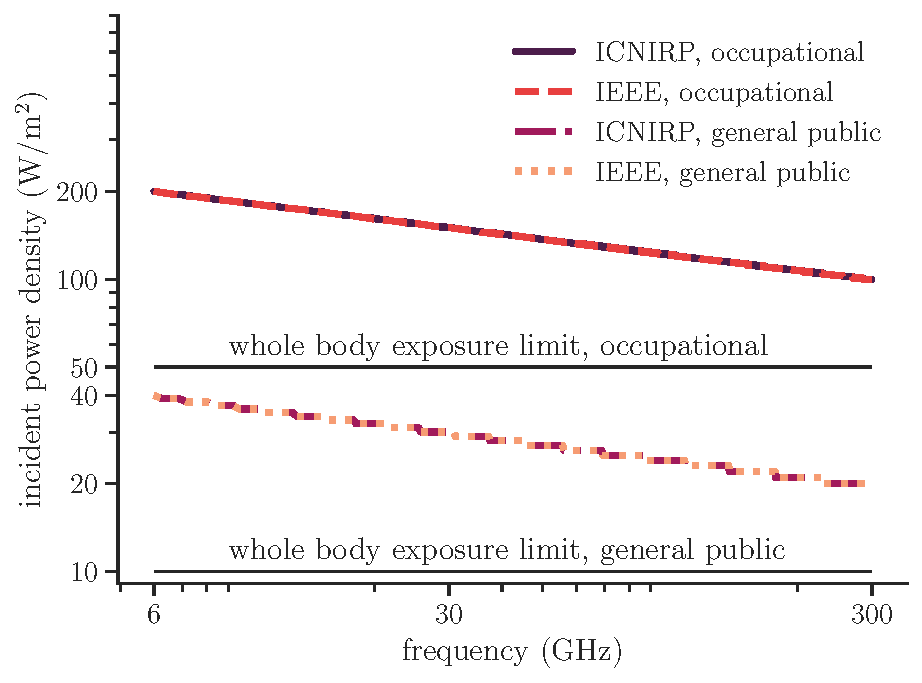
\includegraphics[width=0.8\textwidth]{artwork/reference_levels.pdf}
    \caption{Incident power density as a function of frequency for general public and occupational exposures at \SIrange{6}{300}{\GHz}.}
    \label{fig:reference_levels}
\end{figure}
Constant values of \SIlist{50;10}{\watt\per\m\squared} are prescribed for whole-body exposure in occupational and general public settings, respectively.
For local exposure at \SI{6}{\GHz} within the far-field, compliance is achieved if the peak-spatial \gls{ipd} remains below the specified value.
The plane-wave equivalent \gls{ipd} can be used as a substitute when appropriate.
In the radiative near field, compliance is demonstrated by ensuring that the \gls{ipd} does not exceed the limits.
However, within the reactive near field, compliance cannot be determined based on \gls{ipd} alone; dosimetric values must be assessed instead.

The assessment of cumulative effects from simultaneous exposure to multiple frequency \gls{rf} \gls{emf}s, considering both thermal and electrical stimulation, is out of the scope of this thesis; for details on this subject, refer to~\cite{ICNIRP2020Guidelines, IEEE2019Standard}.
However, it is worth noting that in a recent computational study~\cite{Miura2021Power}, simultaneous exposure at \SIlist{2;28}{\GHz} have been evaluated using realistic antenna models.
It has been shown that the superposition effect is negligible in most cases, except in a very specific situation in which the patch antenna array and inverted-F antenna are separated by less than \SI{50}{\mm} at the antenna-body distance of \SI{5}{\mm}.
